\section{\texorpdfstring{$(2+\epsilon,W_{u,v})$}{(2+epsilon,W{u,v})}-APSP for Weighted Graphs and Unweighted \texorpdfstring{$2$}{2}-APSP}\label{sc:2_W}
In this section, we show that an adapted version of our algorithm returns $(2+\epsilon,W_{u,v})$-approximate distances with improved update time, where $W_{u,v}$ is the maximum weight on a shortest path from $u$ to $v$. 
This result follows by the fact that in this case we do not need to handle the adjacent bunch case, but instead can consider an \emph{overlap} bunch case (see the middle case in Figure~\ref{fig:pivots_allcases}), which leads to an improved running time. 

To make this efficient, there are some additional complications. We introduce a parameter~$\tau$, the \emph{bunch overlap threshold}, which bounds the cluster size. For nodes $w\in B(u)\cap B(v)$ with cluster smaller than $\tau$, we can compute the overlap case. If all nodes in the overlap $B(u)\cap B(v)$ have larger clusters, we obtain an approximate by computing shortest paths from the heavy nodes. More details can be found in \Cref{sec:2_W}.

Moreover, in \Cref{sec:reduction}, we show a general reduction from mixed APSP to purely multiplicative APSP for unweighted graphs. We use this reduction to obtain our unweighted $(2+\epsilon,0)$-APSP result. 

\begin{figure}[htbp!]
    \centering
    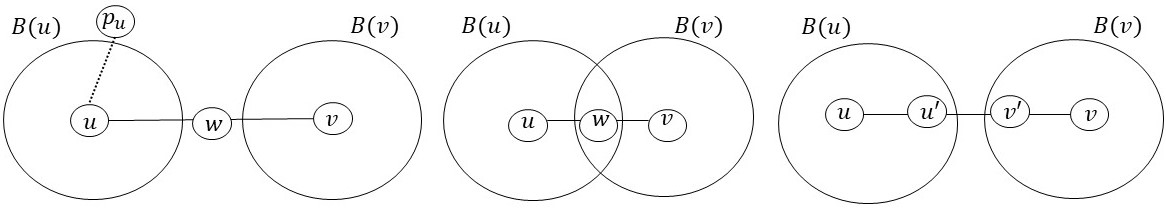
\includegraphics[width=\textwidth]{picture_new}
    \caption{Possible scenarios for the overlap between the bunches $B(u)$ and $B(v)$ and the shortest path $\pi$ from $u$ to $v$.}
    \label{fig:pivots_allcases}
\end{figure}

\subsection{\texorpdfstring{$(2+\epsilon,W_{u,v})$}{(2+epsilon,W{u,v})}-APSP for Weighted Graphs}\label{sec:2_W}
We use the same structure as in \Cref{sec:TZ_2+eps}: we have bunches, and clusters exactly as before. We introduce the parameter $1\leq \tau\leq n$ to be set later. Now we define nodes to be heavy or light based on their cluster size. 
\begin{itemize}
    \item We call a node $ u $ \emph{heavy} if it is or ever was contained in at least $\tau$ approximate bunches $B(v)$, i.e., $u$ is heavy at time $t$ if there is a $t'\leq t$ such that $|C^{(t
     )}(u)|\geq \tau$. If a node is not heavy, we call it \emph{light}. 
    \item Initially, we denoted $V_{\rm{heavy}}$ for the set of heavy nodes, and $V_{\rm{light}}=V\setminus V_{\rm{heavy}}$ for the light nodes. By definition of heavy nodes, a light node can become heavy, but a heavy node can never become light. 
    \item Suppose we have a distance estimate $\delta_H(s,v)$ for all $s\in V_{\rm{heavy}},v\in V$. For each node $u \in V$, the \emph{heavy pivot} $q(u)$ is the closest node in $V_{\rm{heavy}}$ to $u$ according to the distance estimate $\delta_H$
\end{itemize}

We can show that the size of $ V_{\rm{heavy}} $ is bounded. 

\begin{lemma}\label{lm:size_heavy_moved}
 At any given time, with high probability, $ V_{\rm{heavy}} $ has size $\tilde O (\tfrac{n }{p\tau}\log_{1+\epsilon_3}(nW)) $.\label{lm:size_H}
\end{lemma}
\begin{proof}
    Let $B^{(t)}(v)$ and $C^{(t)}(w)$ denote the bunch of $v$  and the cluster of $w$ respectively at time $t$. Since bunch radius $r(v)$ increases by at least a factor $1+\epsilon_3$ if the bunch changes, we have at most $\log_{1+\epsilon_3}(nW)$ different bunch radii. Until the bunch radius increases, the bunch can only lose vertices, which does not contribute to the total size. Since each bunch is of size $\tilde{O}(\tfrac{1}{p})$ with high probability, we obtain that the total size of a bunch over the course of the algorithm is bounded by $\left|\bigcup_{t} B^{(t)}(v)\right|=\tilde{O}\left(\tfrac{\log_{1+\epsilon_3}(nW)}{p}\right)$. Hence we have 
    \begin{align*}
        |V_{\rm{heavy}}|\tau &\leq \sum_{w\in V_{\rm{heavy}}} \tau \\
        &\leq \sum_{w\in V_{\rm{heavy}}} \left| \bigcup_t C^{(t)}(w) \right| \\
        &\leq \sum_{w\in V} \left| \bigcup_t C^{(t)}(w) \right| \\
        &= \sum_{v\in V} \left| \bigcup_t B^{(t)}(v) \right| \\
        &= \tilde O ( \tfrac{n}{p}\log_{1+\epsilon_3}(nW)).
    \end{align*}
    Thus $|V_{\rm{heavy}}| = \tilde O (\tfrac{n }{p\tau}\log_{1+\epsilon_3}(nW))$.\qedhere
\end{proof}

Now we are ready to present our new algorithm. 
\textbf{Algorithm} \DynAPSPtwoW{$V,E,w,p,\tau,\epsilon$}\\
\Initialization{}:

Set $\epsilon_1=\epsilon_2=\epsilon_3=\epsilon_4=\epsilon/3$.
\begin{enumerate}
    \item \textbf{Sampling.} Sample each node with probability $p$ to construct $A$. \label{step:sampling_moved}
    \item \textbf{Distances from $A$.} Compute $(1+\epsilon_1)$-approximate distances $\delta_A(s,v)$ for $s\in A$ and $v\in V$. 
    %Further, for all $v\in V$, initialize a Min-Heap $Q^{\text{dist-from-}A}_v$ that stores the distances $\delta_A(s,v)$ for $s\in A$.
    \item \textbf{Bunches and clusters.} Initialize the algorithm for maintaining the approximate bunches $\tilde B$ and pivots $\tilde p$ according to Lemma~\ref{lm:approx_bunches_on_G}, denoting with $\dLNbunch(v,w)$ the $(1+\epsilon_2)$-approximate distances for $w\in \tilde B(v)$.\\
    Initialize $(1+\epsilon_3)$-approximate bunch radii $r(v)$ with respect to these approximate pivots $\tilde p(v)$.  \label{step:A_MSSP_moved}
    We initialize another approximation to the bunches, denoted by $B(v)$, which will be defined with respect to the bunch radius $r(v)$. Initially, we simply set $B(v)=\tilde{B}(v)$. We let $\delta_B(u,v):=\dLNbunch(u,v)$, and set $\tilde \delta_B(u,v) := (1+\epsilon_4)^{\lceil \log_{1+\epsilon_4}(\delta_B(u,v))\rceil}$. Initialize $V_{\rm{heavy}}:= \{w\in V : |C(w)|>\tau\}$. \label{step:bunches_moved}
    \item \textbf{Distances from $V_{\rm{heavy}}$.} Compute $(1+\epsilon_1)$-approximate distances $\delta_H(s,v)$ for $s\in V_{\rm{heavy}}$ and $v\in V$. Further, for all $v\in V$, we initialize a Min-Heap $Q^{\rm{heavy-pivot}}_v$ that stores $\delta_H(s,v)$ for $s\in V_{\rm{heavy}}$. The heavy pivot $q(v)$ is the minimum entry of $Q^{\rm{heavy-pivot}}_v$. \label{step:H_MSSP_moved}
    \item \textbf{Overlap data structure.} For $u,v\in V$, initialize a Min-Heap $Q^{\rm{overlap}}_{u,v}$, with an entry for each $w\in B(u)\cap B(v)$ that is not contained in $V_{\rm{heavy}}$, with key $\tilde \delta_B(u,w)+\tilde \delta_B(v,w)$.
\end{enumerate}

\noindent\Delete{$u,v$}:\\
\indent \Update{$u,v,\infty$}\\

\noindent\Update{$u,v,w(u,v)$}:
\begin{enumerate}[(1)]
     \item \textbf{Distances from $A$.} For all $s\in A$, run \Update{$u,v,w(u,v)$} on the SSSP approximation denoted by $\delta_A(s,\cdot)$. %If this leads to a change in $d(s,v')$ for some $v'\in V$ we update the corresponding entry in $Q^{\rm{pivots}}_{v'}$. 
    \item \textbf{Distances from $V_{\rm{heavy}}$.} For all $s\in V_{\rm{heavy}}$, run \Update{$u,v,w(u,v)$} on the SSSP approximation denoted by $\delta_H(s,\cdot)$, and update $Q^{\rm{heavy-pivot}}_{\cdot}$ accordingly. 
    % If the minimum entry $d(v',q(v'))$ of $Q^{\rm{heavy-pivot}}_{v'}$ changes:\label{step:update_pivots}
    % \begin{itemize}
    %     \item If $d(v',q(v'))\leq \Theta(d)$, we run \UpdateEstimate{$u',v'$} for all $u'\in V$. 
    % \end{itemize}
    \item \textbf{Update bunches and heaps.} Maintain the bunches and clusters, and update the heaps accordingly. See below for the details.  \label{step:update3_moved}
\end{enumerate}

\noindent\Query{$u,v$}:\\
    Output $\hat d(u, v)$ to be the minimum of 
    \begin{enumerate}[(a)]\setcounter{enumi}{1}
         \item $\min\{ \dLNbunch(u,\tilde p(u))+\delta_A(v,\tilde p(u)),\delta_A(u,\tilde p(v))+\dLNbunch(v,\tilde p(v))\}$;\label{step:pivotW}
        \item $\min\{ \delta_H(u,q(u))+\delta_H(v,q(u)),\delta_H(u,q(v))+\delta_H(v,q(v))\}$;\label{step:quvitW}
        \item The minimum entry of $Q^{\rm{overlap}}_{u,v}$, which gives $\min\{\tilde \delta_B(u,w)+\tilde \delta_B(v,w) : w\in B(u)\cap B(v) \text{ and }w\in V_{\rm{light}}\}$. \label{step:w_light} 
    \end{enumerate}
    
\paragraph{Updating bunches and heaps.}
For completeness, we recall how we update the bunches and clusters. We now maintain different heaps. Again, we maintain the approximate bunches $\tilde B(v)$ for all $v\in V$ by Lemma~\ref{lm:approx_bunches_on_G}. From here maintain the additional approximate bunches $B(v)$ for all $v\in V$ as given in Definition~\ref{def:app_app_bunch}, i.e., 
If there is a change to $\dLNbunch(v',\tilde p(v'))$, do the following two things:
    \begin{itemize}
        \item We check if $\dLNbunch^{(t)}(v',\tilde p^{(t)}(v'))> (1+\epsilon_3)r^{(t-1)}(v')$, and if so we set $r^{(t)}(v')=\dLNbunch^{(t)}(v',p^{(t)}(v'))$ and we set $B^{(t)}(v):=\tilde B^{(t)}(v)$. If not, we set $r^{(t)}(v')=r^{(t-1)}(v')$ and $B^{(t)}(v)=B^{(t-1)}(v)$.
    \end{itemize}
 Let $u'\in V$ be a node for which there is a change to the bunch involving a node $w\in V$. Such a change can be: \ref{case:smaller bunch_copy} $w$ can leave the bunch of $u'$ \ref{case:distance in bunch changed_copy} the distance estimate of $w$ to $u'$ can change while $w$ stays within the bunch, or \ref{case:bigger bunch_copy} $w$ can join the bunch of $u'$. We formalize this as follows, using $\Delta$ to denote which case we are in.
    \begin{enumerate}[(i)]
        \item $w\in B^{(t-1)}(u')$ and $w\notin B^{(t)}(u')$, we set $\Delta=\infty$ to indicate that $w$ is no longer in $B(u')$. \label{case:smaller bunch_copy}
        \item $w\in B^{(t-1)}(u')$ and $w\in B^{(t)}(u')$ with an increased distance estimate $\tilde \delta_B^{(t)}(u',w)$, we set $\Delta=\tilde \delta_B^{(t)}(u',w)$ to be the new distance. \label{case:distance in bunch changed_copy}
        \item \label{case:bigger bunch_copy} $w\notin B^{(t-1)}(u')$ and $w\in B^{(t)}(u')$, we set $\Delta=\tilde \delta_B^{(t)}(u',w)$ to be the distance. 
    \end{enumerate}
        
    
    
    Next, we do the following. 
    If we are in Case~\ref{case:bigger bunch_copy}, we check the cluster size of $w$: if $|C^{(t)}(w)|\geq\tau$, then we add $w$ to $V_{\rm{heavy}}$ and we initialize a SSSP approximation, denoted by $\delta_H(w,\delta)$. Moreover, for each $u'$ in $C^{(t-1)}(w)$ we do the following:
\begin{itemize}
    \item \UpdateOverlapDS{$w,u',\infty$} to remove the corresponding entries $\tilde\delta_B(u',w)+\tilde\delta_B(v',w)$ from the data structures $Q^{\rm{overlap}}_{u',v'}$ for all $v'\in \text{Set}^{\rm{overlap}}_{w,u'}$. Here $\text{Set}^{\rm{overlap}}_{w,u'}$ stores exactly those $v'$ such that there is an entry for $w$ in $Q^{\rm{overlap}}_{u',v'}$. The details on $\text{Set}^{\rm{overlap}}$ can be found together with the definition and total update time of \UpdateOverlapDS are given in Lemma~\ref{lm:min_heap_w}.
\end{itemize}

If we are in Case~\ref{case:bigger bunch_copy} but $|C^{(t)}(w)|<\tau$, or we are in Case~\ref{case:smaller bunch_copy} or~\ref{case:distance in bunch changed_copy}, then we do the following
\begin{itemize}
    \item \UpdateOverlapDS{$w,u',\Delta$} to update the corresponding entries $\tilde\delta_B(u',w)+\tilde\delta_B(v',w)$ in the data structures $Q^{\rm{overlap}}_{u',v'}$ for all $v'\in \text{Set}^{\rm{overlap}}_{w,u'}$. 
\end{itemize}


\paragraph{Distances from $ V_{\rm{heavy}} $.}
First, we note that a node is heavy if it is contained in at least $\tau$ bunches, or equivalently, if $|C(w)|>\tau$. Hence by Lemma~\ref{lm:updatebunches}, we can easily keep track when nodes become heavy and should join $V_{\rm{heavy}}$. 

Next, we use the shortest path algorithm from Lemma~\ref{lm:decr_MSSP}, which we combine with Lemma~\ref{lm:size_heavy}, which states that $V_{\rm{heavy}}$ might be growing over time, but its size is always bounded by $ \tilde O (\tfrac{n }{p\tau}\log_{1+\epsilon_3}(nW)) $. 
Moreover, we maintain the heavy pivots $q(v)$ by maintaining a Min-Heap $Q^{\rm{heavy~pivot}}_v$ for each node $v$, with as entries all nodes $u\in V_{\rm{heavy}}$ with key $\delta_H(u,v)$. Throughout, we will use that we can extract the minimum entry of a Min-Heap in constant time, that we can insert entries in $\log(n)$ time, and that we can edit or delete entries in $\log(n)$ time, given that we know either the key or have a pointer to their location in the Min-Heap. 

This clearly does not incur more than a constant factor in the running time, so together we obtain the following lemma. 

\begin{lemma} \label{lm:heavy_MSSP}
    With high probability, we can maintain $(1+\epsilon_2)$-SSSP from each node in $ V_{\rm{heavy}} $, providing us with $\delta_H(s,v)$ for $s\in V_{\rm{heavy}}$ and $v\in V$. Further, for all $v\in V$, we can maintain heavy pivots $q(v)$ if $d(v,q(v))\leq d$. We can do this in total update time $ \tilde O (\tfrac{m n }{p\tau}\log_{1+\epsilon_3}(nW)) $ if $m=n^{1+\Omega(1)}$ and $\tfrac{n}{p\tau}=n^{\Omega(1)}$, and $ \tilde O (\tfrac{m n^{1+o(1)} }{p\tau}\log_{1+\epsilon_3}(nW)) $ otherwise. 
\end{lemma}


\paragraph{Overlap data structure.}
Now we provide the details of how we maintain the data structure $Q^{\rm{overlap}}_{u,v}$ for all $u,v\in V$, which has entries for all node $w\in B(u)\cap B(v)\cap V_{\rm{light}}$.


% In the next two lemmas we use the fact that $\tilde\delta_B$ changes at most $\log_{1+\epsilon_4}(nW)$ times. Moreover, $v$ can join and leave $B(u)$ at most $\log_{1+\epsilon_3}(nW)$ times, since the bunch $B(u)$ increases at most $\log_{1+\epsilon_3}(nW)$ times.


\begin{lemma}\label{lm:min_heap_w}
   With high probability, we can maintain the data structures $Q^{\rm{overlap}}_{u,v}$ for all $u,v\in V$ in total update time $\tilde O (\tfrac{n\tau }{p} \cdot\log_{1+\epsilon_3}(nW)\log_{1+\epsilon_4}(nW)) $.
\end{lemma}
\begin{proof}
    Conceptually, we initialize a Min-Heap $Q^{\rm{overlap}}_{u,v}$ for each pair $(u,v)\in V\times V$. In practice, we only create the Min-Heap if the first entry is about to be added. This avoids a $\Theta(n^2)$ initialization time. Now fix $v\in V$, and consider the moment we add a node $w$ to $B(v)$. For this data structure, we only need to consider $w\in V_{\rm{light}}$, hence $w$ is part of at most $ \tau $ bunches. When we add $w$ to to $B(v)$, we know it is part of at most $\tau$ other bunches $B(u)$. For each such tuple $(u,w,v)$, we add an entry to the Min-Heap $Q^{\rm{overlap}}_{u,v}$ for $(u,v)$, which stores $w$ with as key the distance estimate $\delta_w(u,v):=\tilde\delta_B(u,w)+\tilde\delta_B(w,v)$. For the total time, notice that for each $v\in V$, we have at most $\tilde O(\tfrac{1}{p})$ different $w\in B(v)$ for which we store at most $\tau$ distances, hence we have total initialization time $ \tilde O (n \cdot \tfrac{1}{p} \cdot \tau) $.
    
    Next, we consider how to update this data structure. Suppose a value $\tilde\delta_B(u,w)$ changed for some $w\in B(u)$ due to an update to the bunches (Lemma~\ref{lm:updatebunches}), then we would need to change the corresponding entries in $Q^{\rm{overlap}}_{u,v}$. Lemma~\ref{lm:updatebunches} gives us $u$, $w$, and the new distance $\tilde \delta_B(u,w)$, which we need to update in all data structures $Q^{\rm{overlap}}_{u,v}$ for which $w\in B(u) \cap B(v)$. Clearly checking all possible~$v$ and looking through the entire $Q^{\rm{overlap}}_{u,v}$ is too slow. Instead, we keep an additional data structure for each node $w\in B(u)$: a set $\text{Set}_{w,u}^{\rm{overlap}}$ that shows for which $v\in V$ it appears in $Q^{\rm{overlap}}_{u,v}$ and a pointer to where in $Q^{\rm{overlap}}_{u,v}$ it appears. We equip this set with the structure of a self-balancing binary search tree, so we have polylogarithmic insertion and removal times. We update this every time the appearance or location in $Q^{\rm{overlap}}_{u,v}$ changes. Now if $\tilde\delta_B(u,w)$ changes due to an update, we can efficiently change the corresponding places in $Q^{\rm{overlap}}_{u,v}$ as follows. 
    
    We define the function \UpdateOverlapDS{$u,w,\Delta$}, where $w$ is an element of $B^{(t-1)}(u)$ and/or $B^{(t)}$, and $\Delta$ is the new value $\tilde\delta_B^{(t)}(u,w)$, or $\infty$ if $w$ is no longer in $B^{(t)}(u)$. Note that we will only call this function for light $w$.\footnote{If $w$ becomes heavy we remove all the corresponding estimates.} \UpdateOverlapDS does one of three things:
    \begin{enumerate}[(i)]
        \item If $\Delta<\infty$, $w\notin B^{(t-1)}(u)$ and $w\in B^{(t)}(u)$. We add the new estimates:\label{step:new}
        \begin{itemize}
            \item We initialize $\text{Set}_{w,u}^{\rm{overlap}}$ to be empty.
            \item For each $v\in C(w)$ we add $\delta_w(u,v):= \tilde\delta_B(u,w)+\tilde\delta_B(w,v)$ to $Q^{\rm{overlap}}_{u,v}$ and store $v$ together with its location in $Q^{\rm{overlap}}_{u,v}$ as entries in $\text{Set}_{w,u}^{\rm{overlap}}$ and $\text{Set}_{w,v}^{\rm{overlap}}$.
        \end{itemize}
        \item If $\Delta<\infty$, $w\in B^{(t-1)}(u)$ and $w\in B^{(t)}(u)$. We update the estimates:\label{step:existing}
        \begin{itemize}
            \item For each entry of $v$ in $\text{Set}_{w,u}^{\rm{overlap}}$, update $\delta_w(u,v)= \tilde\delta_B(u,w)+\tilde\delta_B(w,v)$ in $Q^{\rm{overlap}}_{u,v}$ and update the entries in $\text{Set}_{w,u}^{\rm{overlap}}$ and $\text{Set}_{w,v}^{\rm{overlap}}$ accordingly.
        \end{itemize}
        \item If $\Delta=\infty$, then $w\in B^{(t-1)}(u)$ and $w\notin B^{(t)}(u)$. We remove the corresponding estimates:\label{step:del}
        \begin{itemize}
            \item For each entry of $v$ in $\text{Set}_{w,u}^{\rm{overlap}}$, remove $\delta_w(u,v)$ from $Q^{\rm{overlap}}_{u,v}$ and remove the corresponding entries from $\text{Set}_{w,u}^{\rm{overlap}}$ and $\text{Set}_{w,v}^{\rm{overlap}}$.
        \end{itemize}
    \end{enumerate}

    For the total update time, notice that in total at most $\tilde O(\tfrac{n}{p}\cdot \log_{1+\epsilon_3}(nW))$ nodes get added to a bunch, see Lemma~\ref{lm:size_heavy}. Since we only call this function when the added node $w$ is light at that time, we have $|C(w)|\leq \tau$ and thus step~\ref{step:new} takes $O(\tfrac{n\tau}{p}\cdot \log_{1+\epsilon_3}(nW))$ total update time. For step~\ref{step:existing}, note that the distance can be updated at most $O(\log_{1+\epsilon_4}(nW))$~times and therefore this step has total update time $O(\tfrac{n\tau}{p}\cdot \log_{1+\epsilon_3}(nW)\log_{1+\epsilon_4}(nW))$. Further nodes get deleted from bunches at most as often as they get added, so the total update time of step~\ref{step:del} is dominated by step~\ref{step:new}. We obtain total update time $\tilde O ( \tfrac{n\tau }{p} \cdot \log_{1+\epsilon_3}(nW)\log_{1+\epsilon_4}(nW)) $.
\end{proof}

\paragraph{Update time.}
We summarize the running times in the following lemma. 

\begin{lemma}\label{lm:mult_2W_time}
    With high probability, the algorithm \DynAPSPtwoW has total update time $ \tilde O ((pnm + \tfrac{m n }{p\tau}+\tfrac{n\tau}{ p})\log^2(nW)) $ if $m=n^{1+\Omega(1)}$, $p=n^{\Omega(1)-1}$, $\tfrac{n}{p\tau}=n^{\Omega(1)}$, and $\tau = O(n^{1-\rho})$. Otherwise we have total running time $ \tilde O ((pnm +\tfrac{m n }{p\tau} +\tfrac{n\tau}{ p})n^{o(1)}\log^2(nW)) $.
\end{lemma}
\begin{proof}
    We list the total update times as follows:
\begin{itemize}
    \item \textbf{Sampling.} $O(n)$
    \item \textbf{Distances from $A$.}
    \begin{itemize}
	\item $\tilde{O}(pnm)$ if $m=n^{1+\Omega(1)}$ and $pn=n^{\Omega(1)}$
	\item $\tilde O(pn^{1+o(1)}m)$ otherwise.
    \end{itemize}
    \item \textbf{Bunches and clusters.} 
    \begin{itemize}
	\item $ \tilde O (\tfrac{mn^\rho}{p}) $, for some arbitrarily small constant $\rho$, if $m=n^{1+\Omega(1)}$, 
	\item $\tilde O(\tfrac{mn^{o(1)}}{p})$ otherwise.
    \end{itemize}
 %    \item \textbf{Distances from $ V_{\rm{heavy}} $.}
 %    \begin{itemize}
	% \item $ \tilde O (\tfrac{m n }{p\tau}\log_{1+\epsilon_3}(nW)) $ if $m=n^{1+\Omega(1)}$ and $\tfrac{n}{p\tau}=n^{\Omega(1)}$
	% \item $ \tilde O (\tfrac{m n^{1+o(1)} }{p\tau}\log_{1+\epsilon_3}(nW)) $ otherwise.
 %    \end{itemize}
%   \item \textbf{Overlap data structure.}  $\tilde O (\tfrac{n\tau }{p} \cdot\log_{1+\epsilon_3}(nW)\log_{1+\epsilon_4}(nW)) $
    \item \textbf{Distances from $ V_{\rm{heavy}} $.}
    \begin{itemize}
	\item $ \tilde O (\tfrac{m n }{p\tau}\log_{1+\epsilon_3}(nW)) $ if $m=n^{1+\Omega(1)}$ and $\tfrac{n}{p\tau}=n^{\Omega(1)}$
	\item $ \tilde O (\tfrac{m n^{1+o(1)} }{p\tau}\log_{1+\epsilon_3}(nW)) $ otherwise.
    \end{itemize}
   \item \textbf{Overlap data structure.} $\tilde O (\tfrac{n\tau }{p} \cdot\log_{1+\epsilon_3}(nW)\log_{1+\epsilon_4}(nW)) $.
\end{itemize}

This means for the case that $m=n^{1+\Omega(1)}$, $p=n^{\Omega(1)-1}$, and $\tfrac{n}{p\tau}=n^{\Omega(1)}$, we have total update time
$$ \tilde O ((pnm + \tfrac{mn^\rho}{p}+\tfrac{mn^{\rho}}{p}  + \tfrac{m n }{p\tau}+\tfrac{n\tau}{ p})\log_{1+\epsilon_3}(nW)\log_{1+\epsilon_4}(nW)) = \tilde O ((pnm + \tfrac{mn^{\rho}}{p} + \tfrac{m n }{p\tau}+\tfrac{n\tau}{ p})\log^2(nW)), $$
using that we hide constant factors of $1/\epsilon$ in the $\tilde O$-notation. 
For other choices of $m,n,p$ and $\tau$, we obtain 
$$ \tilde O ((pnm + \tfrac{mn^{\rho}}{p} + \tfrac{m n }{p\tau}+\tfrac{n\tau}{ p})n^{o(1)}\log^2(nW)). $$

If we furthermore assume that $n^\rho = O(n/\tau)$, i.e., $\tau = O(n^{1-\rho})$ for some arbitrarily small $\rho$, then we obtain the simplified version
$$ \tilde O ((pnm +   \tfrac{m n }{p\tau}+\tfrac{n\tau}{ p}\log^2(nW)).$$
For other choices of $m,n,p,$ and $\tau$, we obtain 
\begin{align*}
     \tilde O ((pnm + \tfrac{m n }{p\tau}+\tfrac{n\tau}{ p})n^{o(1)}\log^2(nW)). 
\end{align*}
\end{proof}


    






\thmtwoW*
\begin{proof}
    This result follows from a exchanging the adjacent data structure for the overlap data structure as described in this section. 
    
    By Lemma~\ref{lm:mult_2W_time} we have terms a running time scaling with $pnm+mn/(p\tau)+n\tau/p$. To balance out these terms, we set $mn/(p\tau)=n\tau/p$, hence $\tau=\sqrt{m}$. We set $pnm = mn/(p\tau)$, hence $p=m^{-1/4}$. Note that for $m=n^{1+o(1)}$, this choice for $\rho$ and $\tau$ also satisfies the additional constraints of Lemma~\ref{lm:mult_2W_time}, so in this case we obtain total update time $\tilde O( (pnm+mn/(p\tau)+n\tau/p)\log^2(nW))= \tilde O (nm^{3/4}\log^2(nW))$. If $m=n^{1+o(1)}$ we obtain $\tilde O (n^{1+o(1)}m^{3/4}\log^2(nW))$.
    
    \paragraph{Stretch analysis.} It remains to show that $\hat d(u,v)$ is a $(2+\epsilon,W_{u,v})$-approximation of the distance $d(u,v)$. We do a similar case distinction as in Lemma~\ref{lm:mult_stretch}. Case 1 is exactly the same, since we maintain the relevant estimate through the pivots. For the remainder, we know there is no $w\in \pi$ such that $w\in (B(u)\cup B(v))$, hence the two bunches are adjacent. We know create cases depending on whether the bunches overlap, and if so, if the node in the overlap is heavy or light. 
    
    \begin{itemize}
        \item[Case 2:] $\pi\cap B(u)\cap B(v) =\emptyset$ (the right case in Figure~\ref{fig:pivots_allcases}).\\
        Hence $\pi$ consists of a path from $u$ to $u'\in B(u)$, the edge $\{u',v'\}$ with $v'\in B(v)$, and a path from $v'$ to $v$.
        Since $v'\notin B(u)$, we have $d(u,v')\geq   r(u) \geq \tfrac{\dLNbunch(u,\tilde p(u))}{1+\epsilon_3}$, so $\dLNbunch(u,\tilde p(u))\leq (1+\epsilon_3)d(u,v')$. Similarly, we have $\dLNbunch(v,\tilde p(v))\leq (1+\epsilon_3)d(u',v)$. Combining this, we obtain $\dLNbunch(u,\tilde p(u))+ \dLNbunch(v,\tilde p(v))\leq (1+\epsilon_3)(d(u',v)+d(u,v')) = (1+\epsilon_3)(d(u,v)+w(u',v'))$. Without loss of generality, assume that $\dLNbunch(u,\tilde p(u))\leq  \tfrac{1+\epsilon_3}{2}(d(u,v)+w(u',v'))$.  By Query Step~\ref{step:pivotW} we have:
        \begin{align*} 
            \hat{d}(u,v) &\leq \dLNbunch(u,\tilde p(u))+\delta_A(v,\tilde p(u)) \\
            &\leq \dLNbunch(u,\tilde p(u)) +(1+\epsilon_1)d(v,\tilde p(u))\\
            &\leq \dLNbunch(u,\tilde p(u))+(1+\epsilon_1)(d(u,\tilde p(u))+d(u,v))\\
            &\leq \dLNbunch(u,\tilde p(u))+(1+\epsilon_1)(\dLNbunch(u,\tilde p(u))+d(u,v))\\
            &\leq  (2+\epsilon_1)\tfrac{1+\epsilon_3}{2}(d(u,v)+w(u',v'))+(1+\epsilon_1)d(u,v)\\
            &\leq (2+\tfrac{3}{2}\epsilon_1+\tfrac{1}{2}\epsilon_1\epsilon_3+\epsilon_3)d(u,v)+(1+\tfrac{1}{2}\epsilon_1+\tfrac{1}{2}\epsilon_1\epsilon_3+\epsilon_3)w(u',v') \\
            &\leq (2+\epsilon/2)d(u,v)+(1+\epsilon/2)W_{u,v}\\
            &\leq (2+\epsilon)d(u,v)+W_{u,v}.
        \end{align*}
        \item[Case 3:] 
            There exists $w\in \pi$ such that $w\in (B(u)\cap B(v))$ and $w\in V_{\rm{light}}$ (the middle case in Figure~\ref{fig:pivots_allcases}).\\
            By Query Step~\ref{step:w_light}, we have 
            \begin{align*}
                \hat d(u,v) &\leq \tilde\delta_B(u,w)+\tilde\delta_B(v,w)\\
                &\leq (1+\epsilon_4)(\delta_B(u,w)+\delta_B(v,w))\\
                &\leq (1+\epsilon_4)(1+\epsilon_2)(d(u,w)+d(v,w))\\
                &= (1+\epsilon_2+\epsilon_2\epsilon_4+\epsilon_4)d(u,v)\\
                &\leq (1+\epsilon)d(u,v).
            \end{align*}
            \item[Case 4:] 
            There exists $w\in \pi$ such that $w\in (B(u)\cap B(v))$ and $w\in V_{\rm{heavy}}$ (See Figure~\ref{fig:heavy_pivots2W}).\\
            If $w=q(u)$ then by Query Step~\ref{step:quvitW}, we have $\hat d(u,v)\leq \delta_H(u,q(u))+\delta_H(v,q(u))\leq (1+\epsilon_1)(d(u,q(u))+d(v,q(u))=(1+\epsilon_1)d(u,v)\leq (1+\epsilon)d(u,v)$. If $w=q(v)$, the argument is analogous. 
            
            If $q(u)\neq w \neq q(v)$, then by definition of $q(u)$ and $q(v)$ we obtain $\delta_H(u,q(u))\leq \delta_H(u,w)$ and $\delta_H(v,q(v))\leq \delta_H(v,w)$. So we have $\delta_H(u,q(u))+\delta_H(v,q(v))\leq (1+\epsilon_1)d(u,v)$, hence either $\delta_H(u,q(u))\leq (1+\epsilon)\tfrac{d(u,v)}{2}$ or $\delta_H(v,q(v))\leq (1+\epsilon_1)\tfrac{d(u,v)}{2}$. Without loss of generality, assume $\delta_H(u,q(u))\leq (1+\epsilon_1) \tfrac{d(u,v)}{2}$. Combining this with the triangle inequality, we obtain
            \begin{align*}
                \hat d(u,v) &\leq \delta_H(u,q(u))+\delta_H(q(u),v)\\
                &\leq \delta_H(u,q(u))+(1+\epsilon_1)d(q(u),v)\\
                &\leq \delta_H(u,q(u))+(1+\epsilon_1)(d(u,q(u))+d(u,v))\\
                &\leq (2+\epsilon_1)\delta_H(u,q(u))+(1+\epsilon_1)d(u,v)\\
                &\leq (2+\tfrac{5}{2}\epsilon_1+\tfrac{1}{2}\epsilon_1^2)d(u,v)\\
                &\leq (2+\epsilon)d(u,v).
            \end{align*}  
    \end{itemize}
            
            
    \paragraph{Query time.}
    A query $\Query{u,v}$ consists of the minimum over three values. The first two can be computed in constant time, as the components are all maintained explicitly. The last one is maintained explicitly. This gives us constant query time in total.
\end{proof}

In particular, this means we get $(2+\epsilon,1)$-approximate APSP for unweighted graphs. 

\begin{figure}[htbp!]
    \centering
    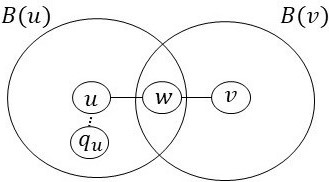
\includegraphics[width=0.35\textwidth]{picture_heavy2W}
    \caption{Possible scenario for the overlap between the bunches $B(u)$ and $B(v)$ and the shortest path $\pi$ from $u$ to $v$ where the estimate can be obtained using heavy pivots $q_u$ and $q_v$.}
    \label{fig:heavy_pivots2W}
    \end{figure}





% \begin{corollary}
%     There exists an algorithm that, given a unweighted graph $G$, maintains $(2+\epsilon,1)$-approximate APSP. The algorithm has total update time $\tilde O( nm^{3/4}\log^2(nW))$ if $m=n^{1+\Omega(1)}$, and $\tilde O( n^{1+o(1)}m^{3/4}\log^2(nW))$ if $m=n^{1+o(1)}$.
% \end{corollary} 
% \begin{proof}
%     We run the algorithm of Theorem~\ref{thm:(2,1)approx} with precision $\epsilon/2$. Denote the distance approximation by $\hat d$, then we have for $u\neq v$:
%     \begin{align*}
%         \hat d(u,v) \leq (2+\epsilon/2)d(u,v)+1+\epsilon/2  \leq (2+\epsilon)d(u,v)+1. 
%     \end{align*}
% \end{proof}

\subsection{Reduction and Unweighted \texorpdfstring{$(2+\epsilon)$}{(2+epsilon)}-APSP}\label{sec:reduction} 
% \section{$(2,0)$-APSP from $(2,k)$-APSP}
Intuitively, we split every edge into $k+1$ edges to form $G'$. Then we compute $(2,k)$-APSP on $G'$, divide the result by $k+1$, and round down to the nearest integer. Because the additive error $k$ is not enough to reach a new node in $G$, we can simply ignore this part of the path. In the following theorem we make this formal. 

\thmreduction*
\begin{proof}
    We construct the auxiliary graph $G'=(V',E')$ as follows.
    \begin{align*}
        V' &:= V \cup \{ \{u,v\}_i : \{u,v\}\in E, i\in\{1, 2, \dots, k\}\}; \\
        E' &:= \bigcup_{\{u,v\}\in E} \{ \{u, \{u,v\}_1\}, \{\{u,v\}_1,\{u,v\}_2\}, \dots, \{\{u,v\}_{k-1},\{u,v\}_k\}, \{\{u,v\}_k, v\} \}.
    \end{align*}
    Clearly this graph has $n+km$ vertices and $(k+1)m$ edges. We compute $(a,k)$-APSP on $G'$ in $\tau_{\mathcal A}(n+km,(k+1)m)$ time using algorithm $\mathcal{A}$, and denote the output by $\delta_{G'}$.
    We set $\delta(u,v) := \lfloor \tfrac{\delta_{G'}(u,v)}{k+1}\rfloor$ for all $u,v\in V$. 

    \textbf{Claim.} $\delta$ gives $(a+(k+2)\epsilon,0)$-approximate APSP on $G$. 

    Let $u,v\in V$. We remark that $d_{G'}(u,v)=(k+1)d_G(u,v)$ for all $u,v\in V$. Which we will use twice. %Let $\pi$ be a $u-v$ path in $G'$. We remark that $\pi\cap V$ corresponds to a $u-v$ path $\overline{\pi}$ in $G$, and that $\pi$ has length at least $(k+1)$ times the length of $\overline{\pi}$,
    
    First, we show that $d_G(u,v)\leq \delta(u,v)$.  This follows from $\delta(u,v) = \lfloor \tfrac{\delta_{G'}(u,v)}{k+1}\rfloor \geq \lfloor \tfrac{d_{G'}(u,v)}{k+1}\rfloor = \lfloor \tfrac{(k+1)d_G(u,v)}{k+1}\rfloor=d_G(u,v)$. 

    Second, we show that $\delta(u,v) \leq (a+(k+2)\epsilon)\cdot d_G(u,v)$. This follows from
    $$\delta(u,v) = \lfloor \tfrac{\delta_{G'}(u,v)}{k+1}\rfloor \leq \lfloor \tfrac{(a+\epsilon)\cdot d_{G'}(u,v)+k}{k+1}\rfloor = \lfloor \tfrac{(a+\epsilon)\cdot (k+1)d_{G}(u,v)+k}{k+1}\rfloor= \lfloor (a+\epsilon)\cdot d_G(u,v) +\tfrac{k}{k+1}\rfloor.$$

    Now if $\epsilon=0$, then $a\cdot d_G(u,v)$ is an integer, hence $\lfloor a\cdot d_G(u,v) +\tfrac{k}{k+1}\rfloor = a\cdot d_G(u,v) $. If $\epsilon>0$, then $\epsilon d_G(u,v)+ \tfrac{k}{k+1}$ can be bigger than $1$ -- if it is not, we are done by the same argument. Now we note that 
    \begin{align*}
        (k+1)\epsilon\cdot d_G(u,v) \geq (k+1)\left(1-\tfrac{k}{k+1}\right) =1.
    \end{align*}
    Hence we obtain 
    \begin{align*}
        \lfloor (a+\epsilon)\cdot d_G(u,v) +\tfrac{k}{k+1}\rfloor &\leq (a+\epsilon)\cdot d_G(u,v) +1 \\
        &\leq (a+\epsilon)\cdot d_G(u,v) + (k+1)\epsilon\cdot d_G(u,v)\\
        &= (a+(k+2)\cdot \epsilon)d_G(u,v).
    \end{align*}
    

    For the claim about dynamic algorithms, note that any update to an edge in $G$, corresponds to updating $k+1$ edges in $G'$. The query consists of computing $\delta(u,v) = \lfloor \tfrac{\delta_{G'}(u,v)}{k+1}\rfloor$, which requires a query to the distance in $G'$ plus constant time operations. 
\end{proof}

In particular, this can give fast algorithms for sparse graphs.
% In the static case, we can obtain (retrieve) the following result. 
% \begin{corollary}
%     There exists an algorithm that, given an unweighted graph $G=(V,E)$, computes $2$-APSP in $\tilde O(m^{5/3})$ time. 
% \end{corollary}
% \begin{proof}
%     We apply the theorem above with the $(2,1)$-APSP algorithm of Baswana, Goyal, and Sen~\cite{BaswanaGS09} which takes $ \tilde O(n'm'^{2/3})$ time (or more precisely, we use the version of \cite{DoryFKNVV23} which avoids a $n'^2$ term. 
% \end{proof}
% For sparse graphs, $m=o(n^{6/5})$, this takes subquadratic time. And for $m=\tilde O(n)$, it matches the conditional lower bounds of \cite{PatrascuRT12,aboud2022stronger}. We note that \cite{DoryFKNVV23} provide the better bound of $\tilde O(mn^{2/3})$, even for weighted graphs, but with a more involved algorithm. 
For the decremental case, we obtain the following result. 
\thmtwoUnw*
\begin{proof}
    We apply the theorem above with the $(2+\epsilon,1)$-APSP of this paper, Theorem 1.2. This takes $\tilde O( nm^{3/4})$ time if $m=n^{1+\Omega(1)}$, and $\tilde O( n^{1+o(1)}m^{3/4})$ time otherwise.
\end{proof}


% \ttodo{Look for $(2,3)$-APSP that we can make decremental. Note that the two subquadratic papers \cite{AkavR20} and \cite{ChechikZ22} give worse bounds (for sparse graphs) than what we have. Maybe adjusting them can give something better, but both results are recent.}
